\begin{frame}{CUBIC: default congestion control today}
    \begin{itemize}
    \item default in Linux (since 2006), OS X (since 2014), Windows (since 2019)
        \begin{itemize}
        \item sysadmin has other options they can configure
        \item can be changed on connection-by-connection basis
        \end{itemize}
    \item big idea: faster increase when further away from window size of last loss
        \begin{itemize}
        \item cubic function with saddle at that window size
        \end{itemize}
    \item intuition: 
        \begin{itemize}
        \item search faster if away from ``steady state''
        \item avoid excess losses from `probing' if at ``steady state''
        \end{itemize}
    \end{itemize}
\end{frame}

\begin{frame}{}
\begin{tikzpicture}
\node (pic) {
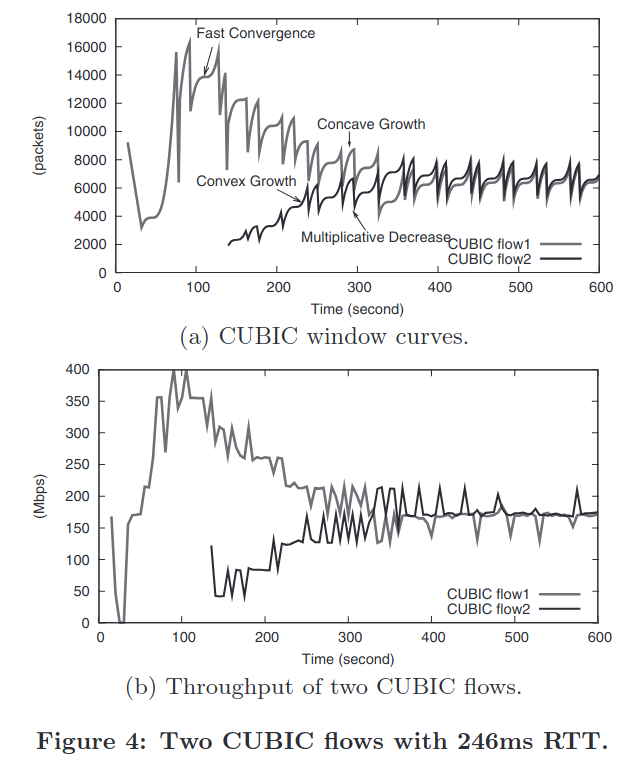
\includegraphics[height=\textheight]{../congest/cubic-fig4}
};
\node[anchor=north west,font=\tiny] at (pic.north east) {
from Ha, Rhee, and Xu, ``CUBIC: A New TCP-Friendly High-Speed TCP Variant''
};
\end{tikzpicture}
\end{frame}
